\chapter{Introduction}
\markright{CHAPTER 1}

%
\section{Background}
% status quo
With the continued urbanization, people keep on migrating from rural areas to urban areas. As a result of this, 54 percent of people worldwide live in urban areas by 2014, this population shift will continues and is predicted to reach 66\% by 2050 \cite{un2014world}. Living in cities is considered much more efficient and convenient than that in rural areas in a variety of ways, as it is easier to provide services when people live closer together. However, cities also change the way that people interact with each other and the environment, which often causes multiple problems. The second UN Conference on Human Settlements in 1996 came to the conclusion that the cities all over the world are facing problems due to urbanization.

% Different situations in developing countries and developed conutries
Although the problems commonly exist all over the world, the type and scale differ from different stages of urbanization. As to developing countries who are now experiencing a rapid change cased by the rapid migrants from rural areas to urban areas, the problems mainly include traffic congestion, disorganization, and pollution. Essentially, most of the problems are caused by the imbalance of demand and supply in land use, resource, and infrastructure. How to satisfy this demand is an important issue that the governments in developing countries have to consider and address. Different from the situation in developing countries, population aging and low birthrate has become the serious problems in developed countries. With a rapidly increasing proportion of aged people in the population, governments are forced to increase expenditure on social security, adding to that the low birthrate, further intensifies the shrinking of working-age population, thus increasing the fiscal burden of governments. How to reduce the public financial expenditure and improve the efficiency of social operation has become a problem that the governments in developed countries have to face. 

% Summary of status quo
In some ways, the problems of the developing countries and the developed countries are different, but in essence, either of them is the problem of sustainability. While governments in the developing world must try to increase the supply of services to satisfy the increasing population, those in the developed world must try to cope with economic slowdown due to decentralization and changing working patterns. Under such a realistic background, a sustainable program for urban planning seems to be necessary. 

% Introduce TOD
With the increasing demand for sustainable development, the concept of TOD was first proposed by Calthorpe, Peter in 1993 \cite{calthorpe1993next}. In urban planning, transit-oriented development (TOD) is a type of urban development that mix residential, business and leisure space within walking distance of public transport. In so doing, TOD aims to increase public transport ridership and by reducing automobile travel, thus promoting sustainable urban growth. As to the precise definition of TOD, while the details vary in scope and specificity, most TOD definitions share several common elements \cite{boarnet1997story,bernick1997transit,megally2001california,cervero2004transit}:

\begin{itemize}
	\item Mixed-use development
	\item Transit stations as cores
	\item Compactness
	\item Pedestrian-friendly
\end{itemize}

% rough definition for TOD
The guidelines of TOD summarized above has received a lot of attention by all levels of governments as the means of mitigating most of the common urban problems, including traffic congestion, air pollution, and incessant sprawl \cite{cervero2002transit}. In a common sense, an area based on TOD typically has a central transit stop (such as a train station, or light rail or bus stop) surrounded by a high-density mixed-use area, with lower-density areas spreading out from this center. The densest areas of a TOD are normally located within a radius of 400 meters to 800 meters (5 minutes to 10 minutes walking duration, varying by different kinds of public transit) around the central transit stop, as this is considered to be an appropriate scale for pedestrians, thus helping solve the last mile problem. 

% Change the objective to rail transit station. Interpret the importance of ridership prediction
With the increase in demand for speed, punctuality and environment protection, urban rail transit has gained popularity by governments, especially in metropolises with high compactness and population density. Add to the continuous extension of city scale and growth in travel demand, more and more TODs are implemented taking rail transit station as the core. With this popularity, it is probably easy to enter a misunderstanding that if the transit station is built, people will come, but the implementation of TOD is not that simple. Because of this, understanding the factors influencing rail transit ridership has become central and fundamental to decisions on urban planning and management under the guidelines of TOD. 

% 
\section{Research purpose}
% propose station level and station-to-station level
What explains rail transit ridership in TOD? As interpreted before, this question is placed in front of us. The answer seems to be both obvious and complex. Every element existing in the catchment area of stations associate with ridership, population, road network, parking, income, transit network, building density, and so on all surely play a role. But the relative importance of these various factors and the internal relations among them are much more complex, and still not well understood \cite{taylor2003factors}. Besides, as transit station is part of transit network rather than an independent existence, once the transit ridership of one station varied, transit ridership of all the other stations connected to that station should vary as well. But the interaction among catchment areas of the stations in the same transit network remains unclear to date.

%  catchment area
We mentioned the term of catchment area above, however, what does it mean in transit ridership analysis? As a general definition, a catchment area is the area from which a city, service or institution attracts a population that uses its services. In the issue of transit ridership analysis, it means a station's primary service area, within which that people are willing to use the station, beyond which land use, travel mode choice, population distribution are unlikely to be influenced by this transit station. The catchment area is thought to be largely determined by people's willingness of walking to transit stations, which, however, vary by people's individual characteristics including trip purpose, age, gender and so on \cite{guerra2013half}. Because of this, the transit catchment area is important and fundamental to the ridership analysis, even the most.

% 基于上述存在的现实问题,我们得出了explain rail transit ridership 这个整体目标。以此为中心,本文针对以下三个问题点进行展开
Based on the interpretation of the real issue above, the research goal of the whole dissertation is defined to \emph{\textbf{explain rail transit ridership}}. Three questions are to be answered in this dissertation.

\begin{itemize}
	\item What explains transit ridership at station level?
	\item What explains transit ridership at station-to-station level?
	\item What explains catchment area?
\end{itemize}

%
\section{Literature review} 
% 首先说明该研究通常包含三个点,然后贴那个大表,从三个点展开
From the research purposes, the literature review is to be extended in terms of method, influencing factor, and catchment area respectively. Table \ref{tab:chp1:Review} gives a brief summary for the literature about transit ridership analysis.

% Table 1
\begin{sidewaystable}[htbp]
	\scriptsize % 该表使用小字体
	\renewcommand{\arraystretch}{0.5} % 重设表间距
	\begin{spacing}{0.5} % 这中间行间距0.5倍
		\centering
		\caption{Summary of some previous studies}
		\label{tab:chp1:Review}
		% 这里的格式控制为限制单元格宽度,自动换行,并居中
		\begin{tabular}{|p{8em}<{\centering}|c|p{5em}<{\centering}|p{5em}<{\centering}|p{5em}<{\centering}|p{5em}<{\centering}|p{5em}<{\centering}|p{5em}<{\centering}|p{5em}<{\centering}|p{5em}<{\centering}|p{5em}<{\centering}|p{5em}<{\centering}|}
			\toprule
			\multicolumn{2}{|c|}{Year} & 2004 & 2004 & 2009  & 2010 & 2011 & 2012 & 2013 & 2013 & 2015  \\
			
			\cmidrule{1-11}
			\multicolumn{2}{|c|}{Author} & Chu & Kuby et al. & Taylor et al. & Sohn and Shim & Gutiérrez et al. & Cardozo et al. & Chakraborty et al. & Zhao et al. & Jun et al.  \\
			
			\cmidrule{1-11}
			\multicolumn{2}{|c|}{Catchment} & $1/4$ mile (400m) walking distance & Half mile (800m) walking distance & N/A & N/A & Distance-decay 800m buffer & 800m walking distance & N/A & 800m radius & 300m, 600m, 900m radius  \\
			
			\cmidrule{1-11}
			\multicolumn{2}{|c|}{Method} & Poisson Regression & WLS & 2SLS & OLS, SEM & OLS & OLS, GWR & OLS, SEM & OLS & OLS, MGWR  \\
			
			\cmidrule{1-11}
			\multicolumn{2}{|c|}{Sample Size} & 2568 & 268 & 265 & 251 & 158 & 190 & 900 & 55 & 442  \\
			
			\cmidrule{1-11}
			\multicolumn{2}{|c|}{Number of Valid Indicator} & 15 & 11 & 8 & 7 & 9 & 4 & 9 & 11 & 11  \\
			
			\cmidrule{1-11}
			\multicolumn{2}{|c|}{Coefficient of determination (Adjusted R2)} & 0.54 & 0.71 & 0.91 & 0.6 & 0.73 & 0.56 & 0.69 & 0.95 & 0.77  \\
			\midrule
			
			% 这里的multirow格式控制,限制宽度自动换行,内容部分加上\centering 可以居中
			\multirow{6}[10]{8em}{\centering{Land use factors}} & Building area & & & & $\bullet$ & $\bullet$ & & $\bullet$ & $\bullet$ & $\bullet$  \\
			\cmidrule{2-11}
			& Hospital & & & & & & & & $\bullet$ &  \\
			\cmidrule{2-11}
			& School/University & & & & $\bullet$ & & & & $\bullet$ &  \\
			\cmidrule{2-11}
			& CBD & & $\bullet$ & & & & & & $\bullet$ &  \\
			\cmidrule{2-11}
			& Land use mix & & & & $\bullet$ & $\bullet$ & $\bullet$ & & & $\bullet$ \\
			\cmidrule{2-11}
			& Other infrastructures & & $\bullet$ & & & & & & $\bullet$ & $\bullet$ \\
			
			\midrule
			\multirow{6}[10]{8em}{\centering{Transit-related factors}} & Accessibility of pedestrian & $\bullet$ & & & & & & $\bullet$ & &  \\
			\cmidrule{2-11}
			& Accessibility of transfer & & $\bullet$ & & $\bullet$ & $\bullet$ & $\bullet$ & $\bullet$ & $\bullet$ & $\bullet$ \\
			\cmidrule{2-11}
			& Road coverage & & & $\bullet$ & $\bullet$ & & & & $\bullet$ &  \\
			\cmidrule{2-11}
			& Parking & & $\bullet$ & & & & & & $\bullet$ &  \\
			\cmidrule{2-11}
			& Service level of public transit & $\bullet$ & $\bullet$ & $\bullet$ & & $\bullet$ & $\bullet$ &       & $\bullet$ & $\bullet$ \\
			\cmidrule{2-11}
			& Locational factor & & $\bullet$ & & $\bullet$ & & & & $\bullet$ &  \\
			\midrule
			
			\multirow{8}[12]{8em}{\centering{Demographic and socioeconomic environment factors}} & Population & & $\bullet$ & $\bullet$ & $\bullet$ & & $\bullet$ & $\bullet$ & $\bullet$ & $\bullet$ \\
			\cmidrule{2-11}
			& Employment & $\bullet$ & $\bullet$ & $\bullet$ & $\bullet$ & $\bullet$ & $\bullet$ & $\bullet$ & $\bullet$ & $\bullet$ \\
			\cmidrule{2-11}
			& Age   & $\bullet$ & & $\bullet$ & & & & & & $\bullet$ \\
			\cmidrule{2-11}
			& Tenant proportion & & $\bullet$ & & & & & & & $\bullet$ \\
			\cmidrule{2-11}
			& Race  & $\bullet$ & $\bullet$ & $\bullet$ & & $\bullet$ & & & &  \\
			\cmidrule{2-11}
			& Income & $\bullet$ & & & & & & $\bullet$ & &  \\
			\cmidrule{2-11}
			& Vehicles holdings & $\bullet$ & & & & & $\bullet$ & $\bullet$ & &  \\
			\cmidrule{2-11}
			& Fare  & & & $\bullet$ & & & & & &  \\
			\bottomrule
		\end{tabular}
	\end{spacing}
\end{sidewaystable}

%
\subsection{Method}
% 定位于交通预测模型
From the view of methodology, exploring and estimating the transit ridership can be treated as part of travel demand forecast \cite{miller1999potential,boyce1994introducing}. There are few fields in urban planning paying more attention to the statistical model for looking into the future than transportation. To date, a host of models have been developed and practiced for the issue of transit ridership, of which the most widely used are the activity-based four-step model and the direct model \cite{mcnally2007four,ewing2010travel}. While either of them works on travel demand forecast, they have different application scenario.

% 吐槽四阶段
Traffic Analysis Zones (TAZs), which is a definition in four-step models, range in size from block groups to census tracts, commonly working at macro scales: corridors, subregions, and stats. The resolution of four-step models tends to be too gross to deal with the issues at neighborhood-scale like TOD \cite{cervero2006alternative}. Even though the four-step model has enjoyed widespread support from decades of use, it was never meant to predict the travel demand at neighborhood-scale taking transit stations as cores, not to mention the estimation of influencing factors on the transit ridership \cite{cervero2006alternative,chu2004ridership,duduta2013direct}. Additionally, in the four-step approach, trip generation stage is usually conducted based on an empirical model using some socioeconomic variables like population, employment, auto ownership, however, in different city cases, the impact of traffic indicators will not be exactly the same \cite{jones1983demand}. It is also unclear whether these selected indicators are significantly related to traffic volume, or whether there is an indeed linear relationship between traffic volume and these selected indicators. 

% 狂吹direct model
Direct models estimates ridership as a function of station environments and transit service features based on observed ridership and statistical data \cite{cervero2006alternative}. With the development of geographic information system (GIS) technology and the richness of digital statistic, direct models have gained popularity in estimating travel demand at neighborhood-scale, most notably for TODs. The advantages of direct models firstly stem from the ease of estimation with data that are readily available to transit agencies. The only critical requirements are GIS, statistics for built-environments around stations, and the corresponding transit ridership \cite{guerra2012half}. The advantages are also reflected in the accuracy of prediction, that much easier and faster than other travel demand models, direct models can also provide strong predictive power \cite{lane2006sketch}. Compared with the disadvantage mentioned in four-step models, since the estimation in direct models is based on the historical statistics, it can justify the importance and validity of indicators that are expected to influence transit ridership \cite{walters2003forecasting}.

%
\subsection{Influencing factor}
% 影响transit ridership的因素分为了3类
Transit ridership is generally thought to be related to land use, transportation environment, or travel preferences \cite{thompson1997achieving}. In 1997, Cervero proposed a three dimension index system (Density, Diversity, and Design) to examine the ridership of transit \cite{cervero1997travel}, which has been generally accepted as a basic principle. In addition, many extensions have also been added to the 3D theory, such as accessibility to the station, connectivity of line, and capacity of station \cite{beimborn2003accessibility,garcia2013walking}. In this study, all the candidate factors expected to influence transit ridership can be classified into three main categories: a. land use factors; b. transit-related factors; c. demographic and socioeconomic environment factors.

% land use factors
Land use includes the buildings or facilities that provide the setting for human activity, and it has been widely proved to have a strong relationship with ridership. Also, land use diversity has a significant effect on ridership since it reflects the balance between traffic demand and supply within the catchment area. Although the definitions of land use diversity are not the same according to different researchers, it is widely accepted that higher diversity tends to result in less transit ridership \cite{cardozo2012application,choi2012analysis,gutierrez2011transit,jun2015land,sohn2010factors,sung2014exploring}.

% transit-related factors
Transit-related factors are important for passengers going to take public transit. Better accessibility is thought to be attractive for passengers living further. The factors for accessibility are commonly described as the number of transfers, network density, number of parking facilities and walking convenience \cite{kuby2004factors,sohn2010factors,taylor2009nature,zhao2014analysis,chu2004ridership}. Also, the type and location of a station can affect accessibility as well. Terminal stations are more attractive for passengers because people can accept to spend more time on getting to a terminal station which is easier to transfer to other line or another mode of transportation \cite{o1996walking}.

% demographic and socioeconomic environment factors
The demographic and socioeconomic environment is an important factor which can reflect the travel preference. Obviously, the resident population and employment-population within the catchment area are crucial factors on ridership of the subway station. Besides, the economic factors also play an important role in ridership. For example, in the area where the car ownership is higher, people are more likely to choose private car than public transit \cite{chiou2015factors,zhao2005transit}; also the higher the percentage of low-income household is, the more likely people tend to take public transit \cite{thompson2012really}. Furthermore, the ratio of apartments and rental house within catchment have been verified being relevant with ridership in some degree \cite{jun2015land}.

%
\subsection{Catchment area}
% historically,buffer area,PCA
An important precondition for investigating factors influencing transit ridership is the definition of the catchment area of a station, which has been interpreted in the part of research purpose. Historically, the determination of transit catchment area was mainly implemented in GIS by creating a distance buffer around the transit station \cite{o1992analysis,hsiao1997use,ayvalik2002heuristic,peng1997simultaneous}. However, since a transit catchment area is determined by the walking distance from the transit station, which is also called pedestrian catchment area (Abbreviated as PCA), a circle buffer area is not adequate for presenting the catchment area. Recent decades, with the development in GIS and the richness in statistics, the application scenario of GIS has progressed far beyond the simple buffering operation \cite{biba2010new,wu2003ptal,jiang2012walk}. Also, many efforts have been made to estimate the real walking distance by importing the data of real road network. According to the existing studies, the PCA generally range from 400 meters to 1000 meters due to different station types, city forms, also travel preference \cite{alshalalfah2007case,guerra2012half,keijer2000people,murray1998public,o1996walking,zhao2003forecasting}.

% 这里给出支持800米, 然后这个800米其实也很不合理
Since difficulties in estimating the accuracy catchment area are still not well addressed, a general 800 meters (half-mile) walking distance, which has been verified to be suitable for most cases, has been widely accepted as a principal reference of the catchment \cite{kuby2004factors,gutierrez2011transit,cardozo2012application,zhao2013influences}. This 800 meters, however, is just a general distance for rail transit stations without considerations of people's individual characteristics and travel preference. The catchment area is mainly determined on the base of questionnaires by asking how far/long did passengers walk to stations, or how far/long are passengers willing to walk to stations \cite{keijer2000people,zhao2003forecasting,garcia2013walking}, while the answers are usually given in a loose way like I remember I walked... or I think I prefer... What's more, the same reasoning has been used to justify other rail transit catchment areas and even in different cities and countries. Till now, restricted by analytical method and data, there are no better options than this general 800 meters walking distance in determining rail transit catchment area, unless doing a large-scale rail transit travel survey which is also thought to be impossible due to excessive costs.

%
\section{Primary research questions}
% 该领域研究大方向的问题
A lot of progress has been made in the research field of transit ridership forecasting, however, some work is still inadequate in the specific problems of the model, influencing factors, and catchment area. From the viewpoint and orientation of this research field, most studies are keeping on mining the problems at station level, but rarely exploring the problems from perspectives of line and network. 

% 针对三个方面的综述,说明每个方面的问题
Specifically, in terms of the model, little progress has been made in the direct model, most existing studies are conducted based on the improvement of regression model but without essential progress. As to influencing factors, scholars have done a thorough job of summary and classification, nevertheless factors behave differently in different cases, the approaches for selecting valid factors towards specific cases are still insufficient. As for the research on catchment area, which even though has been argued very lot to date, the key problems are still not well addressed, either the research perspective or the methodology needs to be further explored.

% 本文将针对的研究点
On the base of fully understanding the existing research, this dissertation will be expanded from the three specific research points corresponding to the research purposes mentioned before.

% 描述的再详细一点
\begin{itemize}
	\item Exploring the approach for screening effective influencing factors.
	\item Shifting the research perspective, trying to describing the relationship between stations and stations.
	\item Exploring the relationship between walking distance and walking preference, and trying to explain the catchment area
\end{itemize}

%
\section{Dissertation organization}
% introduction for study case
The dissertation uses the rail transit system of Fukuoka City, which is the sixth largest city in Japan having a more than 1.5 million population, as the study case. The rail transit system of Fukuoka has 78 rail transit stations, including 27 JR Kyushu stations, 35 subway stations, and 16 West Japan Railway stations. Figure \ref{fig:chp1:ResearchArea} presents the research area and the distribution of rail transit stations. The rail transit system of Fukuoka carries a daily average of more than 0.4 million passengers by 2015 that accounting for more than 20\% in total motorized travel (Ministry of Land, Infrastructure n.d.). Although the rail transit system of Fukuoka is not a large-scale one, it plays a crucial role in public transportation in terms of the city scale and population.

% Figure 1
\begin{figure}[htbp]
	\centering
	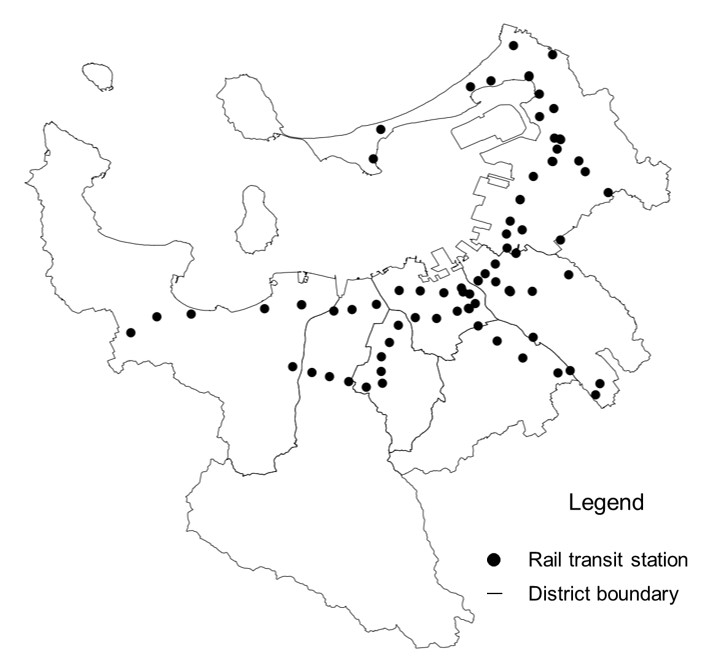
\includegraphics[width=\linewidth]{chp1ResearchArea}
	\caption{Research Area}
	\label{fig:chp1:ResearchArea}
\end{figure}

% organization of dissertation
The content of this dissertation is organized as follow.

\begin{itemize}
	\item \emph{\textbf{Chapter 1}} gives a general introduction to the entire logic and flow with the support of a comprehensive literature review.
	\item \emph{\textbf{Chapter 2}} proposes an approach for selecting the valid indicator used for explain transit ridership, and makes some improvement in the model.
	\item \emph{\textbf{Chapter 3}} explains the influence of land-use patterns on transit ridership at station-to-station level.
	\item \emph{\textbf{Chapter 4}} explores the correlation between surveyed walking duration and people's individual characteristics, thus trying to explain the catchment area.
	\item \emph{\textbf{Chapter 5}} makes a conclusion for the three research point, and prospects the next stage of this research.
\end{itemize}

% 章节划分
\clearpage % 新起一页
\bibliographystyle{apacite}
% \bibliographystyle{IEEEtran}
% 这里需要指定main文件所在路径的相对路径,否则无法读取参考文献。多个bib文件用comma分隔,没有空格
\bibliography{ref}